\chapter{Keypoint Detection}

\begin{introduction}[Keywords]
    \item 角点检测 Corner Detection
    \item 结构张量 Structure Tensor
    \item 特征值分解 Eigenvalue Decomposition
    \item 等变性 Equivariance
    \item 尺度不变性 Scale Invariance
    \item Harris-Laplacian 检测器
    \item 高斯差分 Difference-of-Gaussians (DoG)
\end{introduction}

\section{What Points are Keypoints?}

\begin{enumerate}
    \item Repeatability: 可以在不同的图像中找到相同的点
    \item Saliency: 有趣的点
    \item Quantity: 量大管饱
    \item Accurate localization: 精确定位
\end{enumerate}
Corners 就是这样的 keypoints.

\section{The Basic Idea of Harris Corner}

\begin{figure}[htbp]
    \centering
    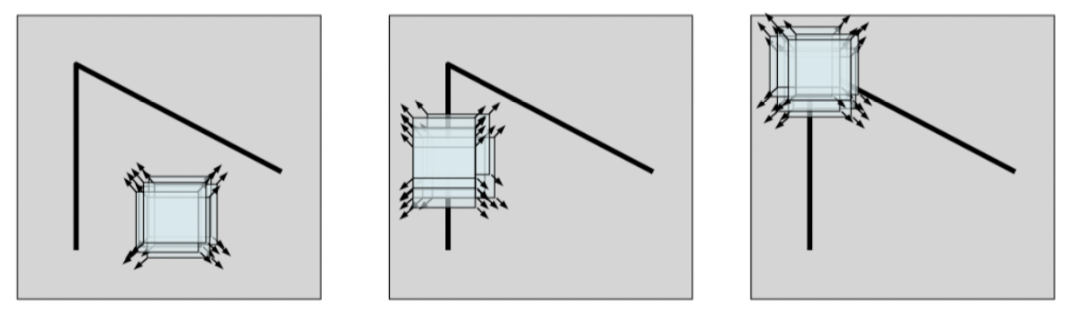
\includegraphics[width=0.8\textwidth]{figures/window_moving.png}
    \caption{移动窗口}
\end{figure}

移动一个窗口,探索窗口内的强度变化。

\begin{itemize}
    \item \textbf{平坦区域 (Flat region)}: 强度变化很小或几乎没有变化。
    \item \textbf{边缘 (Edge)}: 在边缘方向垂直的方向上有显著变化,但沿着边缘方向变化较小。
    \item \textbf{角点 (Corner)}: 在所有方向上的强度变化都很显著。
\end{itemize}

\section{Harris Corner}

我们首先定义强度差异函数 $D_{u,v}(x, y)$,表示对某一像素点在位移 $(u, v)$ 处的变化敏感性:

$$
D_{u,v}(x, y) = \left[I(x + u, y + v) - I(x, y)\right]^2
$$

其中,$I(x, y)$ 是图像在像素点 $(x, y)$ 的强度值 (回忆第一章 Image as a function),$u, v$ 是图像在像素点水平和垂直方向上的位移。

然后,我们定义窗口函数 $w(x, y)$,用于限制计算范围到局部区域:

\begin{equation}
    w(x, y) =
    \begin{cases}
        1, & \text{if } -b < x, y < b \\
        0, & \text{else}
    \end{cases}
\end{equation}

注意到这个函数是一个 \textbf{对称函数}.

继续定义窗口函数的平移版本,其中心位于 $(x_0, y_0)$:

\begin{equation}
    w'_{x_0, y_0}(x, y) = w(x - x_0, y - y_0)
\end{equation}

根据以上定义,我们可以开始推导 $E_{x_0, y_0}(u, v)$, 它的含义是对于以 $(x_0, y_0)$ 为中心,长宽为 $2b$ 的窗口内所有像素点 $(x, y)$, 在位移 $(u, v)$ 作用下的强度变化 $D_{u,v}(x, y)$ 的总和。

\begin{equation}
\begin{aligned}
E_{x_0, y_0}(u, v) &= \sum_{(x, y) \in N} D_{u,v}(x, y) \\
&= \sum_{(x, y) \in N} \left[I(x + u, y + v) - I(x, y)\right]^2 \\
&= \sum_{x, y} w'_{x_0, y_0}(x, y) \cdot \left[I(x + u, y + v) - I(x, y)\right]^2 \\
&= w'_{x_0, y_0} * D_{u,v}
\end{aligned}
\end{equation}

其中 $N$ 是窗口内所有像素点的集合。

\vspace{1em}

接下来我们推导 \textbf{Harris Detector}.

当 $u, v$ 很小 (即位移较小时),对 $I(x + u, y + v)$ 做一阶泰勒展开:

\begin{equation}
    I(x + u, y + v) \approx I(x, y) + I_x \cdot u + I_y \cdot v
\end{equation}

其中:
\begin{itemize}
    \item $I_x = \frac{\partial I}{\partial x}$:图像在 $x$ 方向的梯度。
    \item $I_y = \frac{\partial I}{\partial y}$:图像在 $y$ 方向的梯度。
\end{itemize}

代入平方强度差公式:

\begin{equation}
    D_{u,v}(x, y) = \left[I(x + u, y + v) - I(x, y)\right]^2
    \approx \left(I_x \cdot u + I_y \cdot v\right)^2
\end{equation}

将其写成矩阵形式:

\begin{equation}
    D_{u,v}(x, y) =
    \begin{bmatrix}
        u & v
    \end{bmatrix}
    \begin{bmatrix}
        I_x^2 & I_x I_y \\
        I_x I_y & I_y^2
    \end{bmatrix}
    \begin{bmatrix}
        u \\
        v
    \end{bmatrix}
\end{equation}

将上述结果代入误差函数:

\begin{equation}
    E_{x_0, y_0}(u, v) = w'_{x_0, y_0} * D_{u,v}
\end{equation}

从现在开始,我们省略 $w'_{x_0, y_0}$ 为 $w'$ 来简化表达,利用卷积的性质:

\begin{equation}
    \begin{aligned}
    E(u,v)
    &= w' * D_{u,v}\\
    &= w' \ast \begin{bmatrix} u & v \end{bmatrix} \begin{bmatrix} I_x^2 & I_xI_y \\ I_xI_y & I_y^2 \end{bmatrix} \begin{bmatrix} u \\ v \end{bmatrix}\\
    &= \begin{bmatrix}
        u & v
        \end{bmatrix}
        \left[
        w' *
        \begin{bmatrix}
        I_x^2 & I_x I_y \\
        I_x I_y & I_y^2
        \end{bmatrix}
        \right]
        \begin{bmatrix}
        u \\
        v
        \end{bmatrix}
    \end{aligned}
\end{equation}

注意这里,每个 $I_x, I_y$ 都是一张 \textbf{图像},假设你原图 $I$ 是 $N \times N$ 的,那么

$$
\begin{bmatrix}
    I_x^2 & I_x I_y \\
    I_x I_y & I_y^2
\end{bmatrix}
$$

是 $2N \times 2N$ 的,我们这样实际上是写成了分块矩阵的形式。注意这里 $I_x^2, I_y^2, I_xI_y$ 都是逐点相乘而非矩阵乘法。

如果你对矩阵卷积有所疑惑,那么作为举例,一张 $N \times N$ 的图像 $I_x^2$, 和 $w'$ 卷积的过程可以展开为如下求和:

\begin{equation}
    w' * I_x^2 = \sum_{x, y} w'(x, y) \cdot I_x^2(x, y)
\end{equation}

所以原式中间部分,经过 $w'$ 卷积之后,就会得到一个 $2 \times 2$ 的矩阵。

\begin{equation}
    \begin{aligned}
    E(u,v)
    &= \begin{bmatrix} u & v \end{bmatrix} \begin{bmatrix} w' \ast I_x^2 & w' \ast I_xI_y \\ w' \ast I_xI_y & w' \ast I_y^2 \end{bmatrix} \begin{bmatrix} u \\ v \end{bmatrix}\\
    &= \begin{bmatrix} u & v \end{bmatrix} R^{-1} \begin{bmatrix} \lambda_1 & 0\\ 0 & \lambda_2 \end{bmatrix} R \begin{bmatrix} u \\ v \end{bmatrix}\\
    &= \lambda_1 u_R^2 + \lambda_2 v_R^2
    \end{aligned}
\end{equation}

这里利用了对称矩阵可以进行对角化的性质。$R$ 是一个正交矩阵,且:

\begin{equation}
    \begin{bmatrix} u_R \\ v_R \end{bmatrix} =  R \begin{bmatrix} u \\ v \end{bmatrix}
\end{equation}

所以,最后这里我们判断能量函数大不大,就归结为了判断 

\begin{equation}
    M = \left[
        w' *
        \begin{bmatrix}
        I_x^2 & I_x I_y \\
        I_x I_y & I_y^2
        \end{bmatrix}
    \right]
\end{equation}

的特征值大不大。也即根据这两个特征值的大小可以判断这个点是不是角点。

\begin{figure}[htbp]
    \centering
    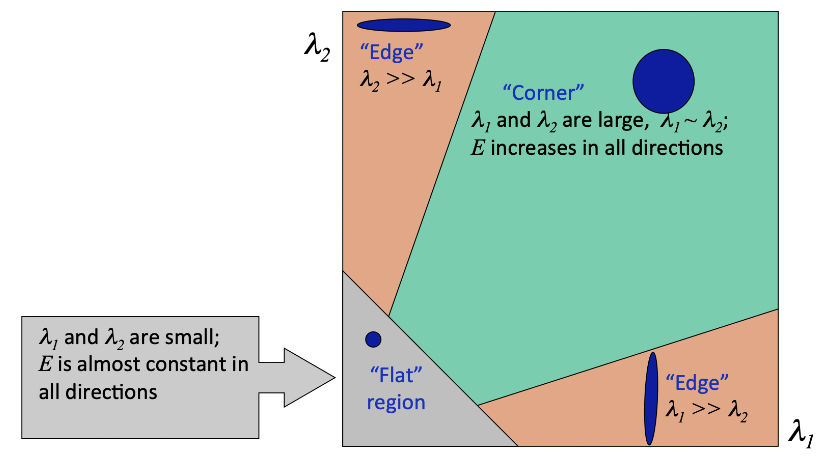
\includegraphics[width=0.6\textwidth]{figures/corner_map.png}
    \caption{特征值大小和这个点的是什么种类的点的关系}
\end{figure}

\newpage

\begin{figure}[htbp]
    \centering
    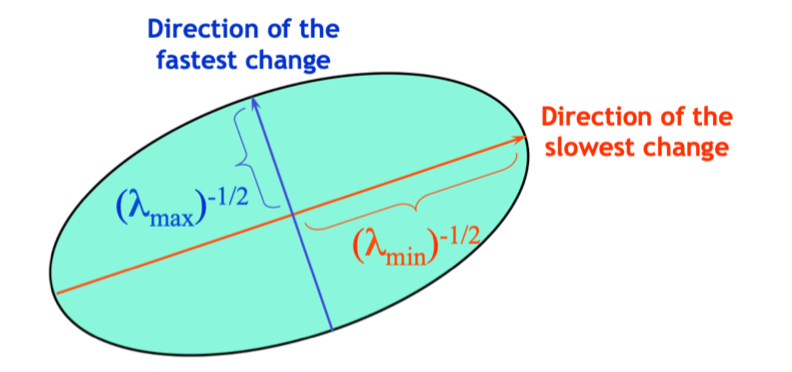
\includegraphics[width=0.6\textwidth]{figures/corner_energy.png}
    \caption{特征值大小和能量函数的关系}
\end{figure}

\begin{proposition}

这个点是角点一般需要满足:

\begin{itemize}
    \item $\lambda_1, \lambda_2>b$: 特征值都大于一个阈值 $b$
    \item $\frac{1}{k}<\frac{\lambda_1}{\lambda_2}<k$: 特征值的比值在 $1/k$ 和 $k$ 之间,确保比例相差不大,否则可能是一个边缘。
\end{itemize}

一个快速的判断公式 (经验公式),引入两个超参 $\alpha$ (用以加权上述两个限制) 和 $t = \frac{b^2}{2}$(阈值):

\begin{equation}
\begin{aligned}
\theta&=\frac 12(\lambda_1\lambda_2-2\alpha(\lambda_1+\lambda_2)^2)+\frac12(\lambda_1\lambda_2-2t)\\
&=\lambda_1\lambda_2-\alpha(\lambda_1+\lambda_2)^2-t\\
&=\det(M)-\alpha\text{Trace}(M)^2-t
\end{aligned}
\end{equation}

推导细节包括:

\begin{itemize}
    \item $\frac 12(\lambda_1\lambda_2-2\alpha(\lambda_1+\lambda_2)^2)$ 这个式子可以粗略的评判 $\frac{1}{k}<\frac{\lambda_1}{\lambda_2}<k$ 的满足程度
    \item 最后一个等号利用了对于对称矩阵(一定可以对角化,对角矩阵又满足 $\det(M) = \prod_{i=1}^n \lambda_i$ 和 $\text{Trace}(M) = \sum_{i=1}^n \lambda_i$)的性质
\end{itemize}

其中 $\alpha\in[0.04,0.06], t\in[0.01,0.03]$.

如果 $\theta$ 大于 0, 也即 $\det(M)-\alpha\text{Trace}(M)^2>t$, 则认为这个点是角点。
\end{proposition}

\begin{note}
基于现在所述窗口函数的 Harris Corner 对平移和 90° 倍数旋转是具有等变性 (equivariant) 的,对非 90° 倍数旋转以及图片缩放不是等变的。

为实现完全的 rotation invariance, 可以用 Gaussian filter 来平滑图像,从而引入其各向同性,使得角点不会因为旋转而改变。

\begin{figure}[htbp]
    \centering
    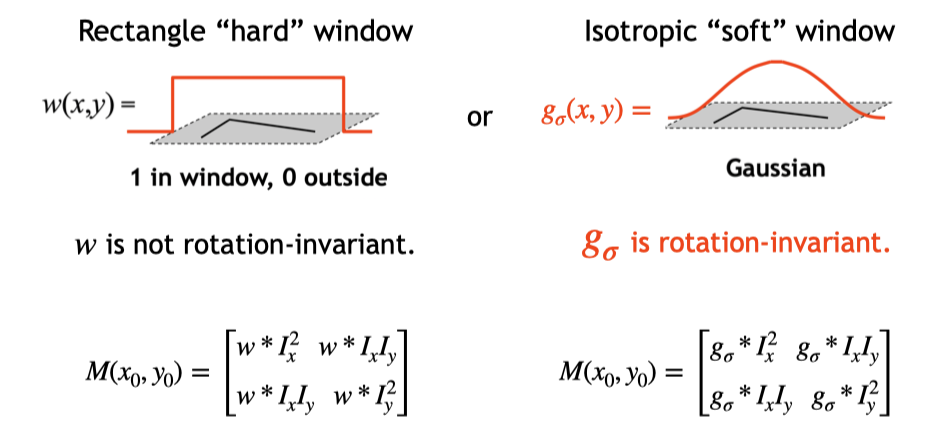
\includegraphics[width=0.6\textwidth]{figures/window-function.png}
    \caption{窗口函数}
\end{figure}


\end{note}
\section{equivariant V.S. invariant}
\begin{definition}

符号定义:

\begin{itemize}
    \item $X \in V$, 表示 $X$ 是一个元素,属于集合 $V$。
    \item $f : V \to V$, 表示 $f$ 是一个函数,输入和输出都来自集合 $V$。
    \item $T : V \to V$, 表示 $T$ 是一个作用在 $V$ 上的变换(例如平移、旋转等)。
\end{itemize}


\textbf{等变 (equivariant)}: 我们称 $f$ 是等变的,如果 $f(T(X))=T(f(X))$(可以交换顺序), 对于 translation 和 rotation 是等变的。

\textbf{不变 (invariant)}: 我们称 $f$ 是不变的,如果 $f(T(X))=f(X)$, 也就是对于不同位置导出的角点还是那样,所以其实我们想要的是等变,也就是对于不同位置导出的角点做了同样的变化。

\begin{remark}
    \begin{itemize}
        \item transition 是平移,它不改变物体本身的上下左右,只是改变其在空间中的位置;
        \item rotation 是旋转,它可能会改变物体本身的上下左右,但不改变其在空间中的位置。
    \end{itemize}
\end{remark}

例子:

\begin{itemize}
    \item 我们希望位置检测是等变的,当图片旋转时,检测到的位置也应该旋转同样的角度。
    \item 我们希望物体分类是不变的,当图片应用了各种数据增强 (旋转、平移、缩放、光照),分类结果不变。
\end{itemize}


\end{definition}

\begin{problem}
    How to prove Harris detector is equivariant?
\end{problem}


只要说明角点检测函数也是 equivariant 即可。

角点检测函数包括了求导和卷积两个操作,显然求导是 equivariant 的,因为导数会随着 transition 和 rotation 做相同的变化。

很有趣的是卷积也是 equivariant 的:当你的 filter function 是 \textbf{各向同性} 的,那么这个卷积就是 equivariant 的;但是如果是一个椭圆形的 window,那这个卷积就不是 equivariant 的了。

显然,卷积对于缩放(zoom in/out)是 invariant 的,因为卷积的窗口大小不变。

注意由于我们对图片进行了离散化(像素化),所以这里关于旋转的等变性可能并不那么严谨。上述说法中也不考虑边缘的问题,假设是无限大的图片。

\newpage

\begin{figure}[htbp]
    \centering
    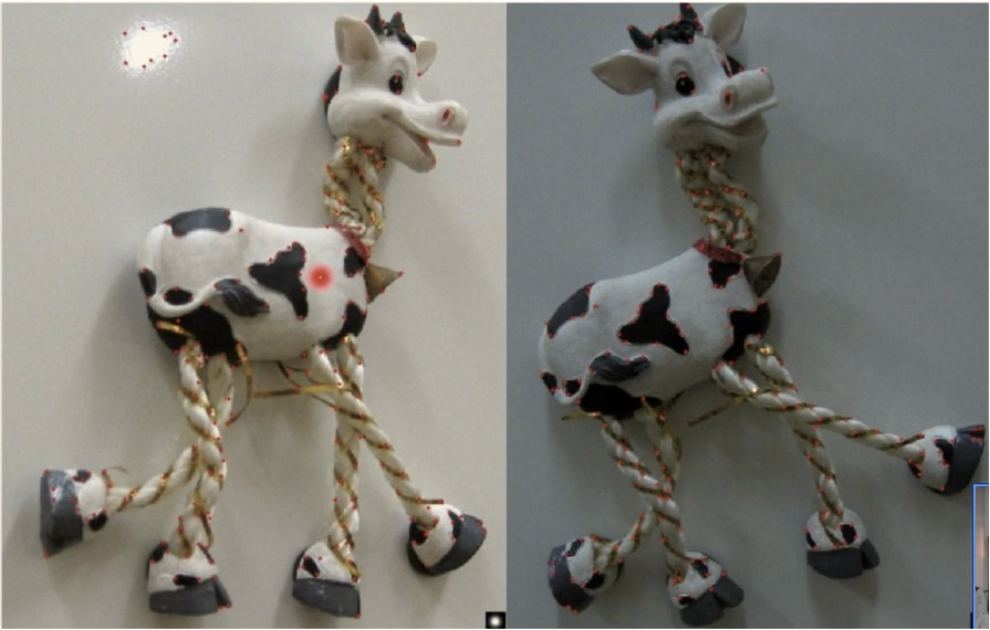
\includegraphics[width=0.6\textwidth]{figures/light_invariant.png}
    \caption{Illumination invariant}
\end{figure}
\begin{remark}
    这个高光说明不是环境 Illumination Invariant 的
\end{remark}


\begin{problem}
    How to do NMS with corner-response-function?
\end{problem}


一个简单的想法:

先给出一个阈值,把所有 response 排序,成为一个 list,从上到下按顺序把这个 pixel 周围的大于阈值的踢出 list.
这个跟之前的 NMS 区别在于之前需要一条边,现在只需要一个点,那么现在比之前踢出的像素点更多。

\section{Scale Invariant Detectors}
\begin{itemize}
    \item Harris-Laplacian: 角点检测器,在空间域用 Harris 角点检测器定位关键点,在尺度域用 Laplacian 响应选择最佳尺度
    \item SIFT: 关键点检测器,直接在空间和尺度域联合搜索关键点,使用 DoG 近似 Laplacian of Gaussian
\end{itemize}
